% !TEX TS-program = pdflatex
% !TEX encoding = UTF-8 Unicode

% This is a simple template for a LaTeX document using the "article" class.
% See "book", "report", "letter" for other types of document.

\documentclass[12pt]{article} % use larger type; default would be 10pt

\usepackage[utf8]{inputenc} % set input encoding (not needed with XeLaTeX)
\usepackage{amssymb}
%%% Examples of Article customizations
% These packages are optional, depending whether you want the features they provide.
% See the LaTeX Companion or other references for full information.

%%% PAGE DIMENSIONS
\usepackage{geometry} % to change the page dimensions
\usepackage{setspace}
\geometry{a4paper} % or letterpaper (US) or a5paper or....
\geometry{margin=1in} % for example, change the margins to 2 inches all round
% \geometry{landscape} % set up the page for landscape
%   read geometry.pdf for detailed page layout information

\usepackage{graphicx} % support the \includegraphics command and options

% \usepackage[parfill]{parskip} % Activate to begin paragraphs with an empty line rather than an indent

%%% PACKAGES
\usepackage{booktabs} % for much better looking tables
\usepackage{array} % for better arrays (eg matrices) in maths
\usepackage{paralist} % very flexible & customisable lists (eg. enumerate/itemize, etc.)
\usepackage{verbatim} % adds environment for commenting out blocks of text & for better verbatim
\usepackage{subfig} % make it possible to include more than one captioned figure/table in a single float
% These packages are all incorporated in the memoir class to one degree or another...

%%% HEADERS & FOOTERS
\usepackage{fancyhdr} % This should be set AFTER setting up the page geometry
\pagestyle{fancy} % options: empty , plain , fancy
\renewcommand{\headrulewidth}{0pt} % customise the layout...
\lhead{}\chead{}\rhead{}
\lfoot{}\cfoot{\thepage}\rfoot{}

%%% SECTION TITLE APPEARANCE
\usepackage{sectsty}
\allsectionsfont{\sffamily\mdseries\upshape} % (See the fntguide.pdf for font help)
% (This matches ConTeXt defaults)

%%% ToC (table of contents) APPEARANCE
\usepackage[nottoc,notlof,notlot]{tocbibind} % Put the bibliography in the ToC
\usepackage[titles,subfigure]{tocloft} % Alter the style of the Table of Contents
\renewcommand{\cftsecfont}{\rmfamily\mdseries\upshape}
\renewcommand{\cftsecpagefont}{\rmfamily\mdseries\upshape} % No bold!

%%% END Article customizations

%%% The "real" document content comes below...

\title{1.3 Bond Enthalpy}
\author{Peter Zhang}
%\date{} % Activate to display a given date or no date (if empty),
         % otherwise the current date is printed 

\doublespacing
\begin{document}
\maketitle

\pagebreak

\tableofcontents

\pagebreak

% start document
\section{Lattice Enthalpy}
\subsection{What is Lattice Enthalpy?}
Lattice enthalpy is the energy required to break 1 mole of an ionic lattice into its individual constituent ions at infinite separation. It is an endothermic process and $\triangle{H}$ is positive.

Lattice enthalpy is useful because it helps us get an accurate answer because ionic reactions are much more than just formation energy. 

\subsection{Lattice Enthalpy Equation}
$$\triangle{H}_{lat} = \triangle{H}_{atomization} + \triangle{H}_i + E + \triangle{H}_e - \triangle{H}_f$$

$\triangle{H}_{atomization}$ = energy required to dissociate a mole of atoms usually from solid to gas

$\triangle{H}_{ionization}$ = energy required to remove one mole of $e^-$ from one mole of gaseous atoms at ground state

E = energy required to break apart bonds (similar to atomization but for non-metals [usually gasses])

$\triangle{H}_{electron\ affinity}$ = energy required to add one mole of $e^-$ to one mole of gaseous atoms at ground state

\subsection{Note about Electron Affinity}

First Electron affinity will always be (-) [exothermic]

After that, most electron affinities will be (+) [endothermic]

\pagebreak

\section{Born-Haber Process}

It is a sequence of steps that allows one to visualize the process in which Lattice Enthalpy is Calculated.

It basically sums up everything in the equation of Lattice Enthalpy

\begin{enumerate}
\item atomization (solid $\rightarrow$ gas)
\item ionization energy
\item electron affinity
\item bond-enthalpy (or atomization for non-metal)
\item enthalpy of formation
\end{enumerate}


\subsection{Example with NaCl}


\begin{figure}[h]
	\centering
	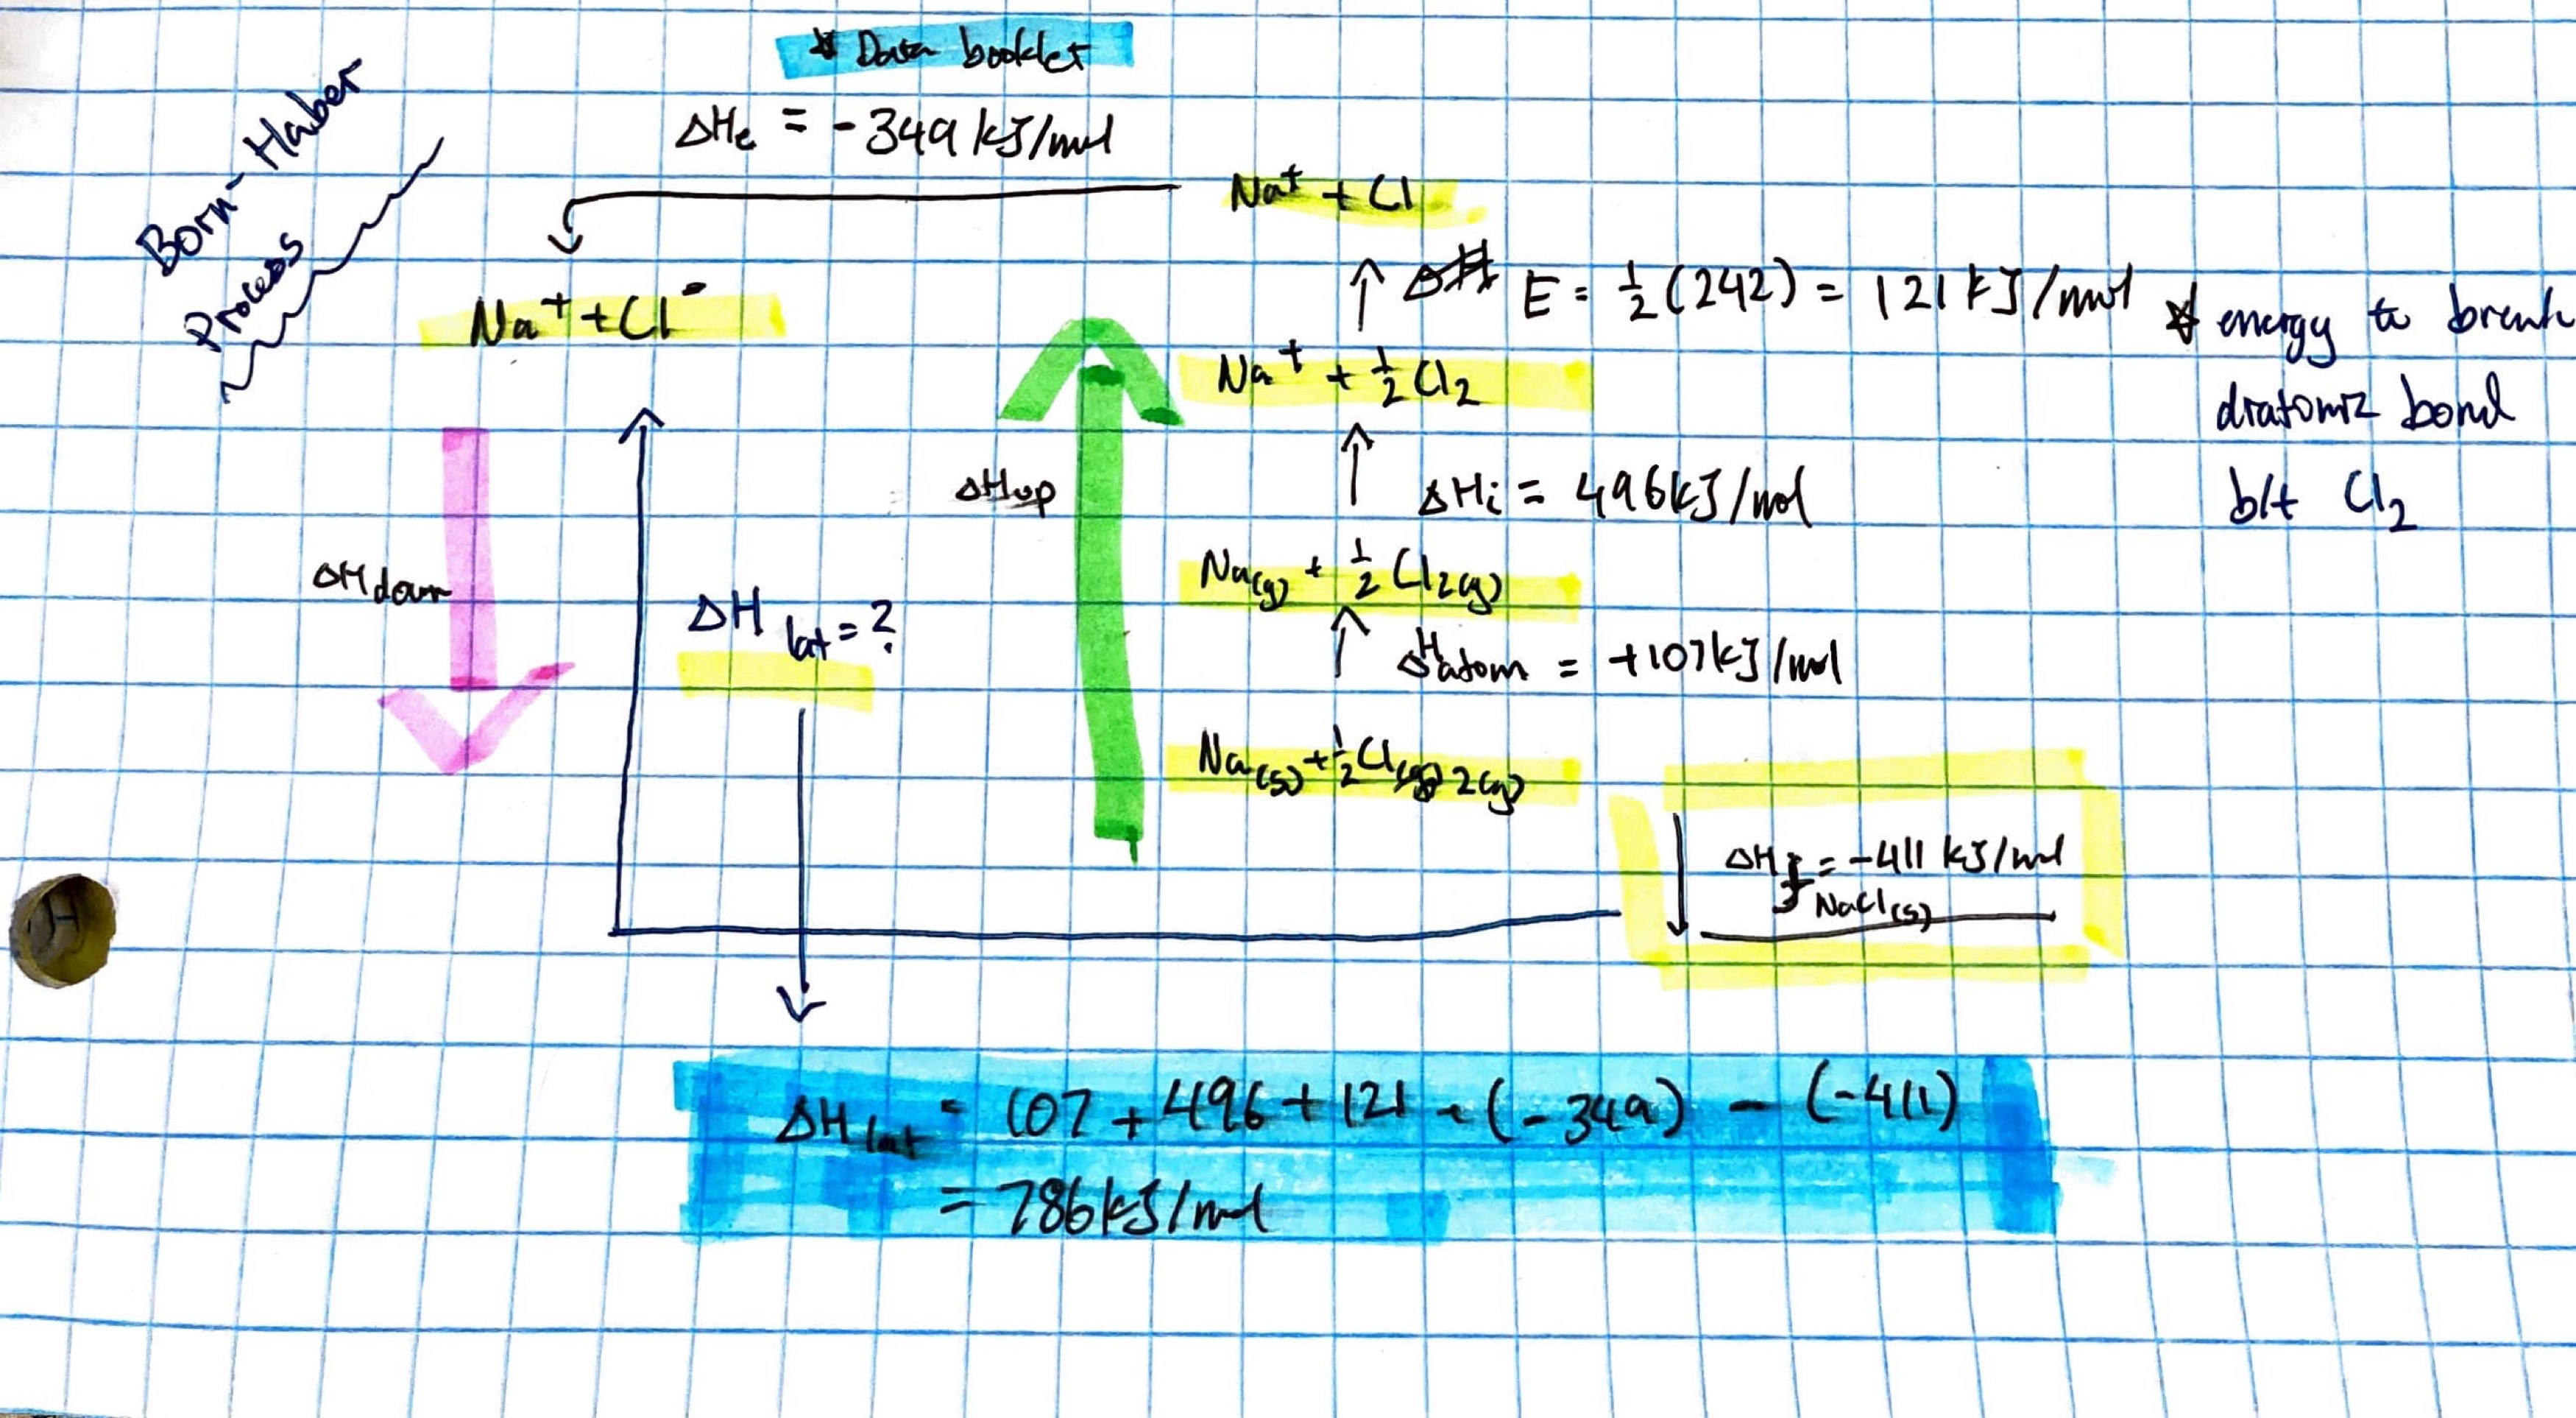
\includegraphics[width=\textwidth]{../images/1.4fig1.JPG}
	\caption{Example for NaCl}
	\label{figure:image}
\end{figure}

The image basically shows you how everything works :l

\begin{itemize}
\item First, the metal is atomized from solid to gaseous state
\item Second, the metal is ionized however many times required
\item Third, the non-metal is atomized and bonds are released
\item Fourth, electron affinity occurs however many times for gas/non-metal
\item Fifth, the enthalpy of formation is taken into consideration
\item Lastly: we find the Lattice Enthalpy: \textbf{Energy required to break one mole of ionic lattice}
\end{itemize}

\subsection{Example with MgO}

\begin{figure}[h]
	\centering
	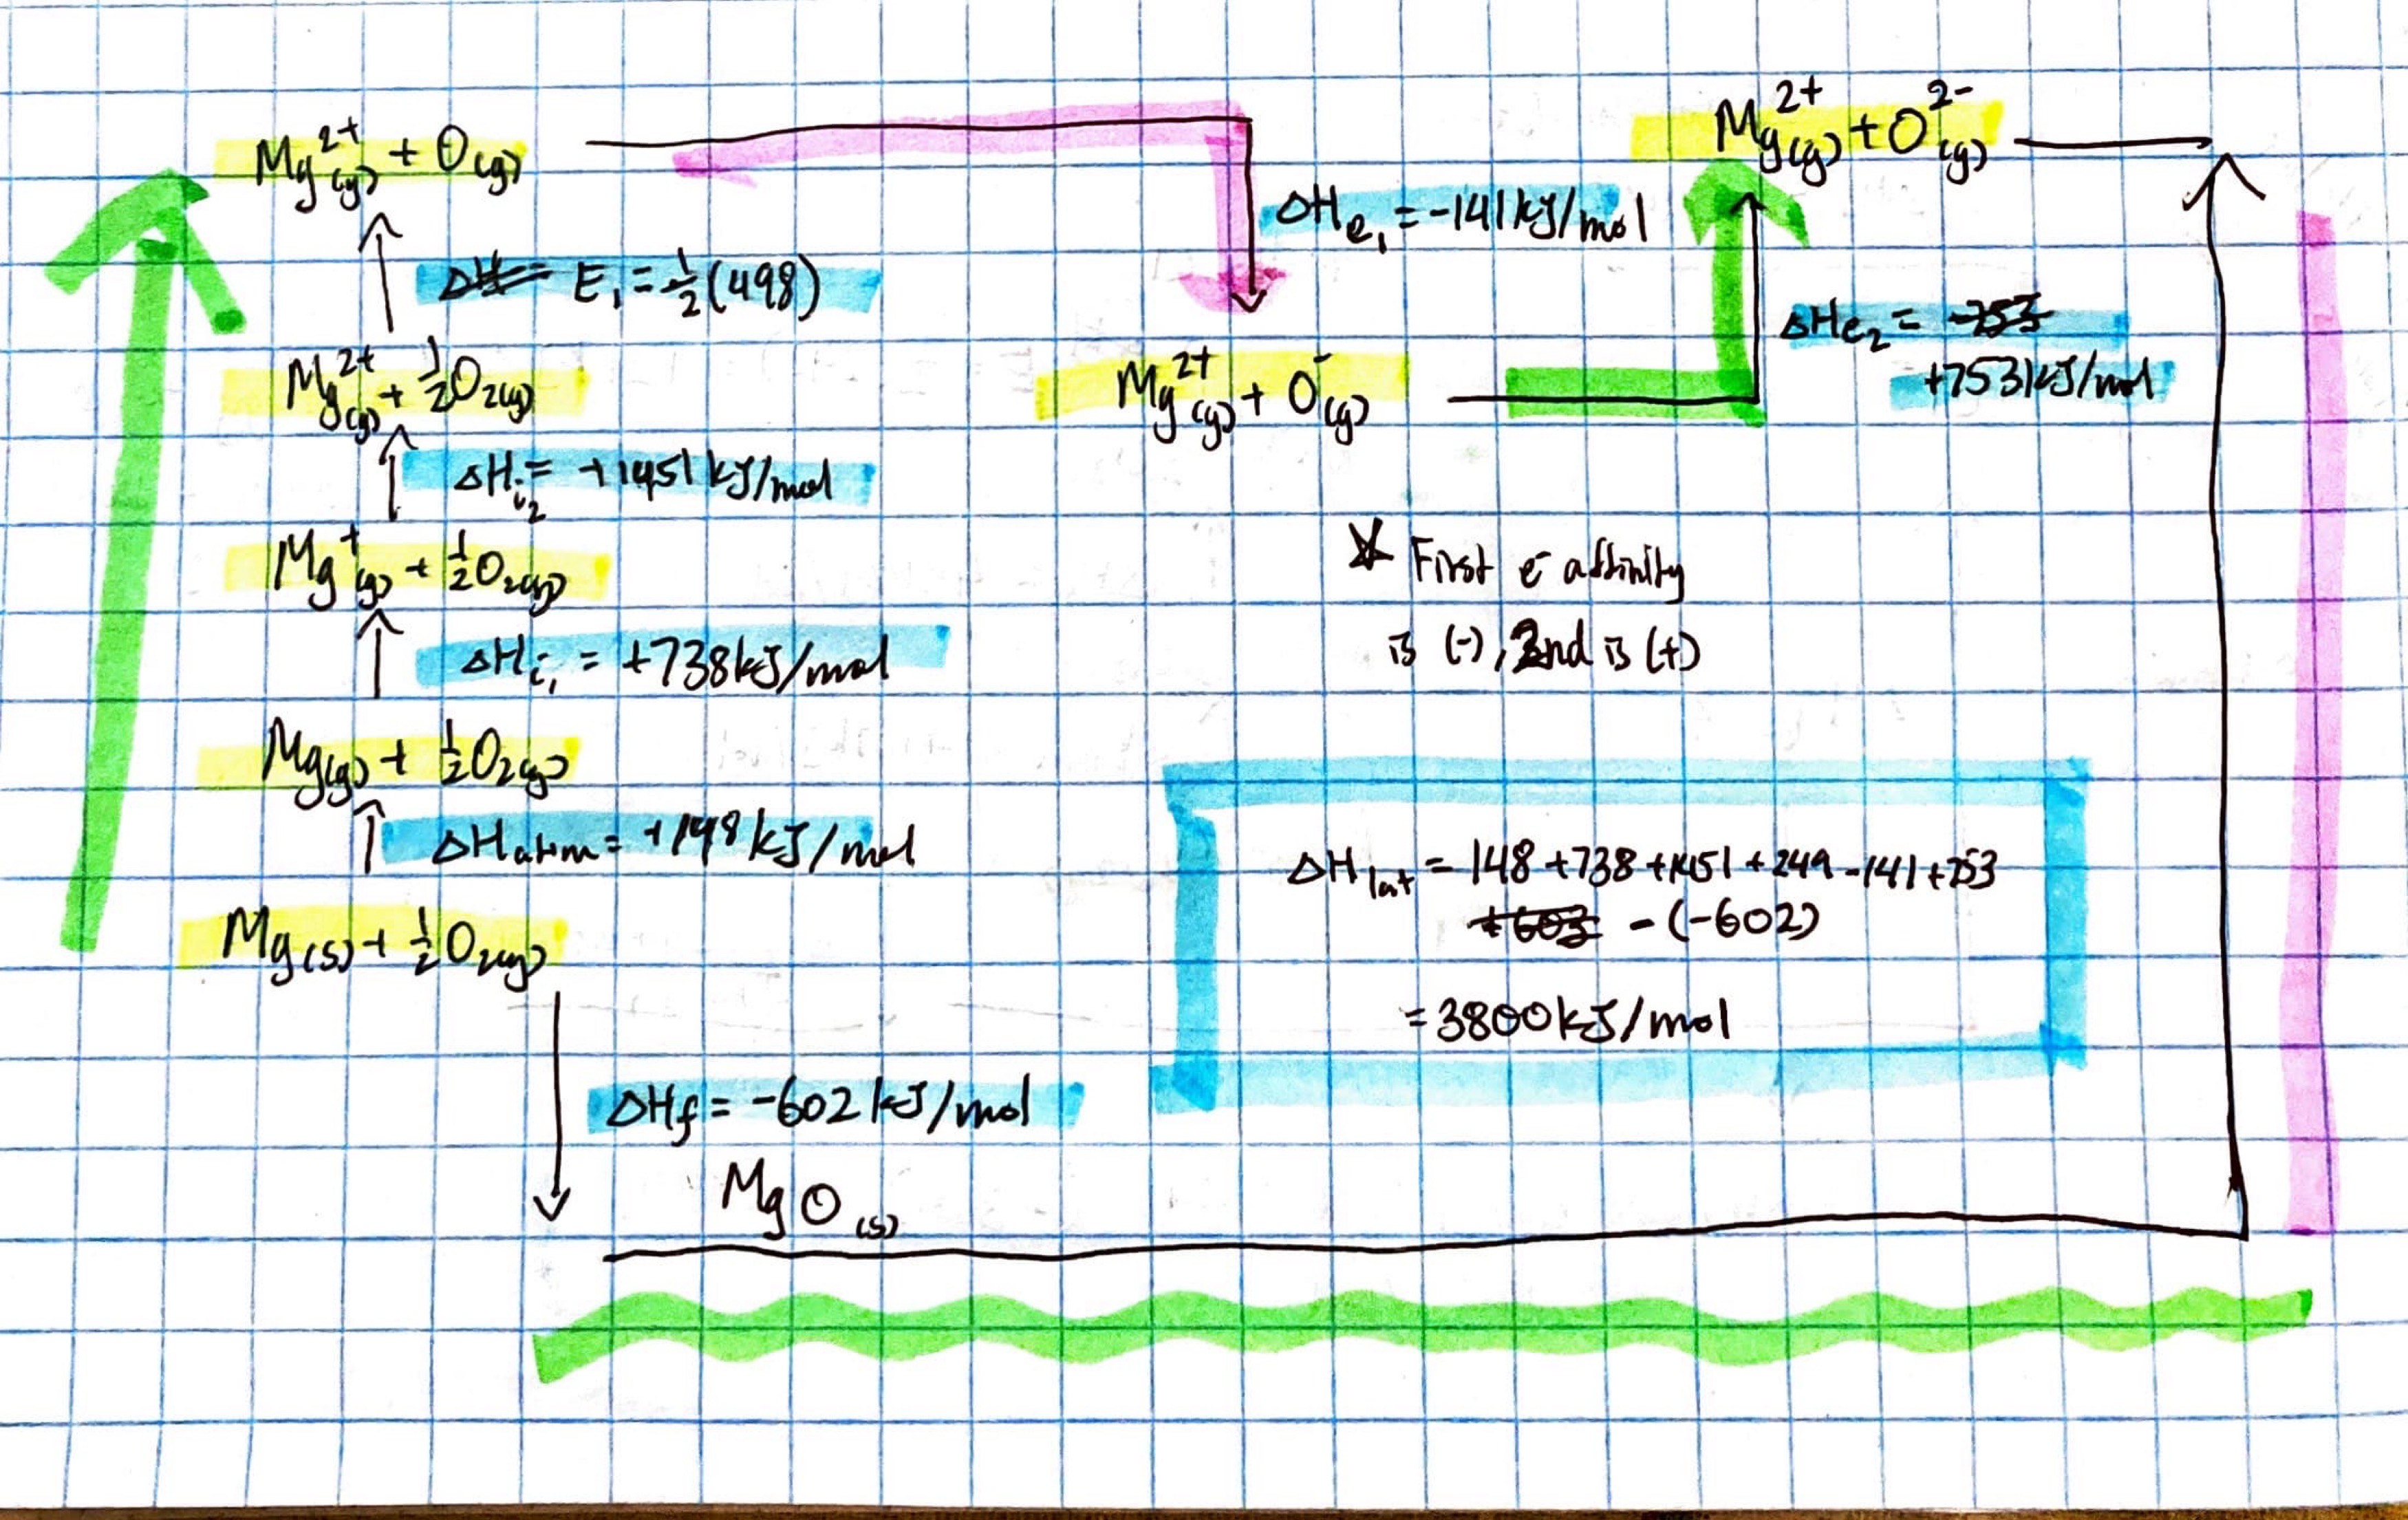
\includegraphics[width=\textwidth]{../images/1.4fig2.JPG}
	\caption{Example for MgO}
	\label{figure:image1}
\end{figure}

Same concept as above


\pagebreak

\section{Enthalpy of Solutions}

This section is about making (aq) solutions and the energy involved in that.

$$\triangle{H}_{solution} \rightarrow \triangle{H}_{lattice} + \triangle{H}_{hydration}$$

The Enthalpy of Solution is the energy required/released when forming ionic solutions. \textbf{Hydration values} can be found in the data booklet. \textbf{Lattice values} can also be found in the data booklet.


\subsection{Example: MgO}

$$MgO_{aq} \rightarrow Mg^{2+}_{aq} + O^{2-}_{aq}$$
\begin{itemize}
\item $\triangle{H}_{MgO_{aq}} \rightarrow \triangle{H}_{lattice} + \triangle{H}_{hydration}$
\item $\triangle{H}_{MgO_{aq}} \rightarrow 3800 + (Mg^{2+} + O^{2-})$
\item $\triangle{H}_{MgO_{aq}} \rightarrow 3800 + [-1983 + (-600)]$
\item $\triangle{H}_{MgO_{aq}} \rightarrow 1237kJ/mol$
\end{itemize}

\subsection{Example: $AlCl_3$}

$$AlCl_{3(aq)} \rightarrow Al^{3+}_{aq} + 3Cl^{-}_{aq}$$

\begin{itemize}
\item $\triangle{H}_{AlCl_{3aq}} \rightarrow \triangle{H}_{lattice} + \triangle{H}_{hydration}$
\item $\triangle{H}_{AlCl_{3aq}} \rightarrow 2700 + [-4741 + (3 * -359)]$
\item $\triangle{H}_{AlCl_{3aq}} \rightarrow -3118kJ/mol$
\end{itemize}


\end{document}














